\documentclass{article}

% Impostare la lingua italiana
\usepackage[italian]{babel}
\usepackage{listings}
\usepackage{xcolor}
\usepackage{geometry}
\usepackage{mdframed}
\usepackage{fontawesome5}
\usepackage{hyperref}
\usepackage{clipboard}
\usepackage{tcolorbox}

\newenvironment{commandbox}{%
  \begin{tcolorbox}[colback=white,colframe=black!50!white,sharp corners,width=\textwidth]%
  \ttfamily
}{%
  \end{tcolorbox}%
}




% Definizione dello stile per il codice Java
\lstdefinestyle{mystyle}{
    language=Java,
    basicstyle=\small\ttfamily,
    keywordstyle=\color{blue},
    commentstyle=\color{green!40!black},
    stringstyle=\color{orange},
    breaklines=true,
    frame=single,
    numbers=left,
    numberstyle=\tiny,
    captionpos=b,
    tabsize=4
}

% Define margins
\setlength{\topmargin}{-1.0cm}
\setlength{\oddsidemargin}{0.1cm}
\setlength{\textwidth}{16.5cm}
\setlength{\textheight}{23.0cm}

\usepackage{graphicx} %LaTeX package to import graphics
\graphicspath{{images/}} %configuring the graphicx package

% Define header and footer
\usepackage{fancyhdr}
\pagestyle{fancy}
\fancyhf{}
\lhead{{
\includegraphics[height=.65cm]{images/uniparthenope.png}}}
\rhead{\textbf{\textit{Progetto Starship}} }
\cfoot{\textbf{\textit{\thepage}}}
% \lfoot{\textbf{\textit{Page \thepage/\pageref*{LastPage}}}}
% \rfoot{\textbf{\textit{Alejandro Romero Prieto}}}
% \renewcommand{\footrulewidth}{0.7pt}
\renewcommand{\headrulewidth}{0.7pt}
\setlength{\headheight}{23pt}

% This is to define a style with no footer for the table of contents
\fancypagestyle{nofooter}{%
  \fancyfoot{}%
}

% To manage references
\usepackage{natbib}

% Hyperlinks setup
\usepackage{hyperref}

\begin{document}

% Title Page %%%%%%%%%%%%%%%%%%%%%%%%%%%%%%%%%%%%%%%%%%%%%%%%%%%%%%%%%%%%%%%%%%%%%%%%%%%%%%%% 

\begin{center}
\vspace*{3\baselineskip}


\includegraphics[width=0.8\textwidth]{images/uniparthenope.png}\\
\vfill

{\huge \textbf{Reti di calcolatori}}

\vspace*{3\baselineskip}

{\LARGE \textbf{Progetto Starship}}

\begin{large}
\vspace*{2\baselineskip}

\vspace*{2\baselineskip}

%Submitted by \\[\baselineskip]
{\Large Vincenzo De Candia \\ \par} % Editor list
{{ 0124002539}}\\[2cm] % Editor affiliation


\vspace*{4\baselineskip}

% 	{\scshape  \today} \\[0.3\baselineskip] % Year published
{\large Università degli Studi di Napoli Parthenope}\par % Publisher

\thispagestyle{empty} 

\end{large}
\end{center}
\pagebreak


% Contents %%%%%%%%%%%%%%%%%%%%%%%%%%%%%%%%%%%%%%%%%%%%%%%%%%%%%%%%%%%%%%%%%%%%%%%%%%%%%%%%%%%%%%%%

% \lhead{\emph{Contents}} % Set the left side page header to "Contents"
\tableofcontents
    \thispagestyle{nofooter}
    %\include{abstract/abstract}
    \cleardoublepage
    \typeout{}

\pagebreak

% Descrizione del progetto 1 %%%%%%%%%%%%%%%%%%%%%%%%%%%%%%%%%%%%%%%%%%%%%%%%%%%%%%%%%%%%%%%%%%%%%%%%%%%%%%%%%%%%%%%%%

\setcounter{page}{1}

\section{Descrizione del progetto}
\label{sec:Descrizione del progetto}

Il progetto si concentra sullo sviluppo di un sistema per la navigazione sicura di una navicella spaziale attraverso una tempesta di meteoriti. La navicella agisce come il client, mentre il server gestisce il settore spaziale dei meteoriti. Il server ha lo scopo di generare 5 meteoriti con posizioni random mentre la navicella deve evitare i meteoriti generati dal server e nel caso in cui si trovassero nella stessa posizione il client riceve un alert ed ha 3 secondi per spostarsi per evitare la collisione.
La comunicazione avviene tramite il protocollo UDP (User Datagram Protocol), che consente una trasmissione veloce e non affidabile dei dati.



% Descrizione e schema dell'architettura 2
%%%%%%%%%%%%%%%%%%%%%%%%%%%%%%%%%%%%%%%%%%%%%%%%%%%%%%%%%%%%%%%%%%%%%%%%%%%%%%%%%%%%%%%%%

\section{Descrizione e schema dell'architettura}
\label{sec:Descrizione e schema dell'architettura}

\begin{figure}[htbp] % Imposta la posizione dell'immagine (h=here, t=top, b=bottom, p=page)
  \centering % Centra l'immagine
  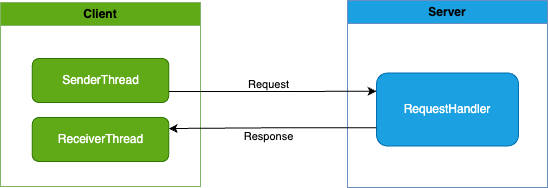
\includegraphics[width=0.8\textwidth]{images/SchemaUDP.png} % Inserisce l'immagine, sostituisci "nome_file" con il nome del file dell'immagine
  \caption{Architettura client-server} % Aggiunge una didascalia all'immagine
  \label{fig:label} % Aggiunge un'etichetta all'immagine per riferimenti incrociati
\end{figure}

\subsection{Server}
\begin{itemize}
    \item Il server UDP si mette in ascolto su una porta specifica per ricevere pacchetti dai client.
    \item Quando riceve un pacchetto, crea un nuovo thread di gestione della richiesta (RequestHandler) per gestire la connessione con il client.
    \item Ogni thread di gestione della richiesta (RequestHandler) si occupa di ricevere i dati dal client, elaborarli e inviare eventuali risposte.
\end{itemize}

\subsection{Client}
\begin{itemize}
    \item Il client UDP utilizza due thread separati: uno per inviare dati al server (SenderThread) e uno per ricevere dati dal server (ReceiverThread).
    \item Il thread SenderThread si occupa di inviare dati al server, mentre il thread ReceiverThread si occupa di ricevere dati dal server.
    \item Entrambi i thread sono eseguiti contemporaneamente per consentire al client di gestire l'invio e la ricezione di dati in modo concorrente.
\end{itemize}
\pagebreak

% Dettagli implementativi dei client/server 3
%%%%%%%%%%%%%%%%%%%%%%%%%%%%%%%%%%%%%%%%%%%%%%%%%%%%%%%%%%%%%%%%%%%%%%%%%%%%%%%%%%%%%%%%%
\section{Dettagli implementativi dei client/server}
\label{sec:Dettagli implementativi dei client/server}
\subsection{ServerUDP}

Il server crea un'istanza di \textbf{DatagramSocket} associata a una porta specifica per ascoltare le richieste in arrivo dai client.
Il server UDP ascolta continuamente per i pacchetti in arrivo utilizzando il metodo \textit{receive() }della classe \textbf{DatagramSocket}. Quando arriva un pacchetto, il server istanzia un nuovo oggetto \textbf{RequestHandler} in un thread separato per gestire la richiesta del client. Questo consente al server di continuare ad ascoltare per ulteriori richieste mentre gestisce quelle esistenti.
\textbf{RequestHandler} elabora i dati ricevuti dal client, determinando il tipo di messaggio ricevuto tramite la classe \textbf{JSONHandler}. Se il messaggio è "mapDimension", il gestore di richieste imposta la larghezza della mappa del gioco e imposta la variabile booleana \textit{TRUE} per permettere al ciclo while di essere eseguito ed inviare dati al client. Se il messaggio è "game over", il gestore di richieste interrompe il thread di invio.
I dati vengono incapsulati in pacchetti Datagram e inviati al client tramite il metodo \textit{send()} del socket.

\subsection{ClientUDP}

All'avvio del gioco viene istanziata la classe \textbf{UDPClient}.
Nel costruttore della classe, vengono inizializzati i parametri del server (hostname e porta) insieme all'oggetto \textbf{EnemySubject}, che gestisce gli oggetti nemici all'interno del gioco. Viene anche creato il socket Datagram utilizzato per la comunicazione con il server e inizializzati i thread \textbf{senderThread} e \textbf{receiverThread}.
Il thread \textbf{senderThread} invia messaggi al server tramite pacchetti datagram.
Il client può inviare solo 2 messaggi, il primo comprende le dimensioni della mappa mentre il secondo contiene un messaggio di game over.


\pagebreak

% Parti rilevanti del codice sviluppato %%%%%%%%%%%%%%%%%%%%%%%%%%%%%%%%%%%%%%%%%%%%%%%%%%%%%%%%%%%%%%%%%%%%%%%%%%%%%%%%%%%% 
\section{Parti rilevanti del codice sviluppato}
\label{sec:Parti rilevanti del codice sviluppato}
\begin{lstlisting}[style=mystyle, caption={ServerUDP}, label={lst:codice}]

/* Il server UDP utilizza un thread separato per gestire ogni richiesta attiva proveniente dai client. Quando il server riceve una nuova richiesta da un client, controlla se quel client ha già una richiesta attiva. Se il server trova una richiesta attiva associata al client, interrompe il thread associato a quella richiesta precedente. Questo viene fatto per evitare conflitti e sovrapposizioni nel processamento delle richieste da parte dello stesso client. Successivamente, il server istanzia un nuovo oggetto per gestire la nuova richiesta e lo memorizza in un HashMap, associandolo al client che ha inviato la richiesta. */

byte[] receiveBuffer = new byte[1024];
DatagramPacket receivePacket = new DatagramPacket(receiveBuffer, receiveBuffer.length);
socket.receive(receivePacket); 

InetAddress clientAddress = receivePacket.getAddress(); // Get the client's address
int clientPort = receivePacket.getPort();

String clientString = clientAddress.toString() + clientPort;

if (clientThreads.containsKey(clientString)) {
    Thread previousThread = clientThreads.get(clientString);
    if (!previousThread.isInterrupted()) {
        previousThread.interrupt();
    }
}

RequestHandler requestHandler = new RequestHandler(receivePacket, socket);
clientThreads.put(clientString, requestHandler);
requestHandler.start();
                
\end{lstlisting}


\begin{lstlisting}[style=mystyle, caption={Request handler} , label={lst:codice}]
/*
Il thread del server UDP, una volta avviato, esegue il metodo receive() per elaborare il pacchetto ricevuto dal client. Se il server riceve un pacchetto contenente le dimensioni della mappa, aggiorna una variabile di stato (running) a true. Questo segnala al thread di avviare un ciclo while successivo, che consentirà al server di inviare pacchetti contenenti posizioni casuali di meteoriti al client ogni 2 secondi.
*/
@Override
    public void run() {
        receive(); // Receive and process data from the client
        if (running) {
            try {
                while (!Thread.currentThread().isInterrupted()) {
                    // Generate random positions for enemy entities
                    for (int i = 0; i <= numberPacket; i++) {
                        Random random = new Random();
                        int randomValue = random.nextInt(getDimensionWidth());
                        JSONObject enemy = new JSONObject();
                        enemy.put("positionX", randomValue);
                        enemy.put("positionY", 0);
                        send(enemy); // Send the position of enemy to the client
                    }
                    Thread.sleep(2000); // Pause for 2 seconds before sending the next batch of positions
                }
            } catch (InterruptedException | IOException e) {
                // Thread interrupted, likely due to stop() method call
                System.out.println("Thread interrupted");
            }
        }
    }

    private void receive() {
        JSONObject jsonObject = new JSONHandler(receivePacket).getJsonObject();
        String typeMessage = jsonObject.getString("message");
        switch (typeMessage) {
            case "mapDimension":
                // Set the dimension width and allow the sender thread to start
                dimensionWidth = jsonObject.getInt("width");
                running = true;
                break;
            case "game over":
                // Received game over message, stop the sender thread
                System.out.println("STOP");
                running = false;
                break;
            default:
                break;
        }
    }

    public void send(JSONObject jsonObject) throws IOException {
        InetAddress clientAddress = receivePacket.getAddress();
        int clientPort = receivePacket.getPort();
        DatagramPacket sendPacket = new JSONHandler(jsonObject, clientAddress, clientPort).getDatagramPacket();
        socket.send(sendPacket); // Send the packet to the client
    }

\end{lstlisting}

\begin{lstlisting}[style=mystyle, caption={Client SenderThread}, label={lst:codice}]
try {
            while (!Thread.currentThread().isInterrupted()) {
                if (thereIsDataToSend()) {
                    JSONObject jsonObject;
                    jsonObject = getJSON();
                    DatagramPacket datagramPacket = new JSONHandler(jsonObject, inetAddress, serverPort).getDatagramPacket();
                    socket.send(datagramPacket);
                }
            }
        } catch (IOException e) {
            System.err.println("Error while sending data: " + e.getMessage());
            Thread.currentThread().interrupt();
        } finally {
            socket.close();
        }

\end{lstlisting}

\begin{lstlisting}[style=mystyle, caption={Client ReceiverThread}, label={lst:codice}]
@Override
    public void run() {
        try {
            while (!Thread.currentThread().isInterrupted()) {
                List<AObject> enemyList = new ArrayList<>();
                enemyList.add(receive());
                enemySubject.setStateEnemyList(enemyList);
            }
        } catch (IOException | ClassNotFoundException e) {
            System.out.println("Receiver closed");
        }
    }

    public AObject receive() throws IOException, ClassNotFoundException {
        byte[] receiveBuffer = new byte[1024];
        DatagramPacket receivedPacket = new DatagramPacket(receiveBuffer, receiveBuffer.length);
        socket.receive(receivedPacket);
        JSONObject jsonObject = new JSONHandler(receivedPacket).getJsonObject();
        int x = jsonObject.getInt("positionX");
        int y = jsonObject.getInt("positionY");
        return new Enemy(x, y);
    }

\end{lstlisting}


\pagebreak

% Manuale utente con le istruzioni su compilazione ed esecuzione %%%%%%%%%%%%%%%%%%%%%%%%%%%%%%%%%%%%%%%%%%%%%%%%%%%%%%%%%%%%%%%%%%%%%%%%%%%%%%%%%%%% 
\section{Manuale utente con le istruzioni su compilazione ed esecuzione}
\subsection{Installazione di Maven su MacOS}

 Prima di installare Maven bisogna installare homebrew


\begin{commandbox}
\begin{verbatim}
/bin/bash -c "$(curl -fsSL https://raw.githubusercontent.com/Homebrew/
install/HEAD/install.sh)"
\end{verbatim}
\end{commandbox}

Una volta installato Homebrew, è possibile installare Maven eseguendo il seguente comando:
\begin{commandbox}
\begin{verbatim}
brew install maven
\end{verbatim}
\end{commandbox}

Dopo l'installazione, verifichiamo che Maven sia stato installato correttamente eseguendo:

\begin{commandbox}
\begin{verbatim}
mvn -version
\end{verbatim}
\end{commandbox}


\subsection{Installazione di Maven su Linux}
Su Linux, si utilizza il gestore di pacchetti apt per installare Maven. Ecco come farlo:

\begin{commandbox}
\begin{verbatim}
sudo apt update
sudo apt install maven
\end{verbatim}
\end{commandbox}


Dopo l'installazione, verifichiamo che Maven sia stato installato correttamente eseguendo:

\begin{commandbox}
\begin{verbatim}
mvn -version
\end{verbatim}
\end{commandbox}

\subsection{Compilazione ed esecuzione del client}
Per compilare ed eseguire il client eseguire il seguente comando:

\begin{commandbox}
\begin{verbatim}
cd Starship
mvn clean javafx:run
\end{verbatim}
\end{commandbox}

\subsection{Compilazione ed esecuzione del server}

Per compilare il server eseguire il seguente comando:
\begin{commandbox}
javac -cp ServerUDP/lib/json-20200518.jar:. ServerUDP/src/Main.java\newline
javac -cp ServerUDP/lib/json-20200518.jar:. ServerUDP/src/JSONHandler.java \newline
javac -cp ServerUDP/lib/json-20200518.jar:. ServerUDP/src/UDPServer.java \newline
javac -cp ServerUDP/lib/json-20200518.jar:. ServerUDP/src/RequestHandler.java
\end{commandbox}

Per avviare il server eseguire i seguenti comandi:
\begin{commandbox}
\begin{verbatim}
cd ServerUDP/src
java -cp ServerUDP/lib/json-20200518.jar:. Main
\end{verbatim}
\end{commandbox}



\clearpage
\end{document}
